\subsection{Migración}
\subsubsection{Contexto social}
El contexto social en el caso de la investigación, como ya se presento anteriormente, abarca desde la parte histórica en la que se conjugaron muchos poblados y etnias en la zona, hasta hoy en día, donde mediante todas las mezclas, avances tanto tecnológicos como sociales, el entorno ha cambiado, y las tradiciones, costumbres y cultura en general, lo han echo de igual manera, todo esto se tratará de describir en los siguientes apartados. 

\subsubsection{Estructura social}
``La sociedad centromexicana durante el Posclásico Tardío tenía una estructura jerárquica. La familia era el núcleo básico. Los conjuntos de familias formaban una agrupación que los españoles llamaban la cuadrilla. Varias cuadrillas formaban un barrio. Los barrios se unían dentro de los señoríos. Algunos señoríos formaban confederaciones estratégicas.'' \citep[p. 156]{Otomies} hoy en día, la estructura familiar continua siendo hasta cierto punto, similar a la que se describe, ya que todavía se suele contar con un sistema patriarcal, en el que el hombre de la casa provee el sustento a toda la familia, y enseña a los hijos varones el oficio o da la oportunidad a que se desenvuelvan en el entorno laboral, mientras las mujeres se dedican al cuidado de la casa y a la enseñanza a las niñas del hogar.

Pasada cierta edad, el hombre del hogar, suele dividir sus tierras y repartirlas entre sus hijos varones. Esperando que puedan construir en ese espacio su hogar y el de su familia, creando divisiones cada vez mas chicas ya que este proceso se hace exponencial durante muchas generaciones.

\subsubsection{Avances}
Los avances tecnológicos, globalización e industrialización junto con diferentes aspectos que han surgido durante el tiempo en México así como los cambios culturales que estas han traído fueron causando de forma gradual que las comunidades originarias fueran desplazadas junto con sus saberes y tradiciones a algo marginal y que las grandes ciudades solo conocen como algo de lo que tienen una cierta clase de orgullo debido a los medios, pero desconocen en profundidad los aspectos que estas comunidades viven en su día a día y los cambios que están causando la pérdida del patrimonio tanto inmaterial como material que vienen de estas comunidades, el valle del Mezquital no se queda atrás en este aspecto, ya que mucha gente conoce la región por su producción de pulque, maguey y su cultura gastronómica, que fomentan el turismo tanto interno como externo del país, pero este turismo, crea una imagen ilusoria que, en algunos casos, genera una visión diferente de lo que se consideraría el vivir bien y vivir mal causando que las personas internas de las comunidades, salgan en busca de ese vivir bien, provocando la migración de sus miembros, específicamente hablando, ``la mayor parte de jóvenes en el Valle del Mezquital buscan migrar a Estados Unidos en busca de mejores ingresos que puedan mandar a sus familias para sustentar mejor sus gastos'' \citep{baez2012pueblos}.

Junto con todos estos cambios surge una contradicción entre la nueva tipología de vivienda y la tradicional, en la que se enfrentan estos dos tipos de conocimiento y nuevas ideas, pero esto puede suponer algo bueno, ya que una contradicción siempre ayuda a la evolución de alguna de las partes y ``en la sociedad humana, al igual que en la naturaleza, un todo único invariablemente se divide en diferentes partes; sólo hay diferencias en el contenido y la forma bajo condiciones concretas diversas. Siempre existirán opuestos como lo correcto y lo erróneo, lo bueno y lo malo, lo hermoso y lo feo. Solo cuando hay diferenciación y lucha, puede haber evolución. La verdad se desarrolla a través de su lucha con la falsedad'' \citep{mao1974cinco}. Pero esto no quiere decir que la visión de un tipo de arquitectura se vuelva unilateral, sino que se puedan distinguir las ventajas y desventajas que  cada sistema constructivo aporta al contexto inmediato donde se planea implementar y con esto, poder llegar a la mejor decisión de construcción, la mas viable y con esto no generar cambios radicales en la forma de habitar de las personas que vayan a ocupar el inmueble.

Dejando como referencia: ``Se considerará Patrimonio cultural: Los monumentos: obras arquitectónicas, de escultura o de pintura monumentales, elementos o estructuras de carácter arqueológico, inscripciones, cavernas y grupos de elementos, que tengan un valor universal excepcional desde el punto de vista de la historia, del arte o de la ciencia''\citep{UNESCO1972}.


\subsubsection{Habitantes}
Como ya se menciono con anterioridad, la migración es un factor de suma importancia en muchas de las localidades de la región pero esto no es forzosamente un factor que sea rotundo en el cambio ideológico de todos los migrantes, como ejemplo tenemos a un habitante de la comunidad \emph{El Deca} el cual a pesar de haber estado 8 años en el extranjero, al regresar a su lugar de origen y sufriendo una experiencia familiar adversa, pudo visualizar el valor de sus tradiciones de una manera excepcional. Esto le sirvió como impulso para generar y proponer una iniciativa para que las costumbres y tradiciones, en especial las de los artesanos, fueran revalorizadas y puestas en practica de una mejor manera.

Plácido junto a su grupo de artesanos al que denominaron Wäda que significa maguey en lengua Hñähñu y con ayuda de una asociación civil llamada \emph{Cooperación Comunitaria}, lograron generar un taller llamado \emph{Xido Ngu}, que funcionara como resguardo de estas tradiciones y cultura, incluso respetando la tipología constructiva en el que su uso Tepetate, siendo la única diferencia que el aglomerante entre cada piedra, fue con cemento en lugar de lodo pero, respetando la tradición del techo a base de pencas de maguey.

\begin{figure}[ht]
    \center
    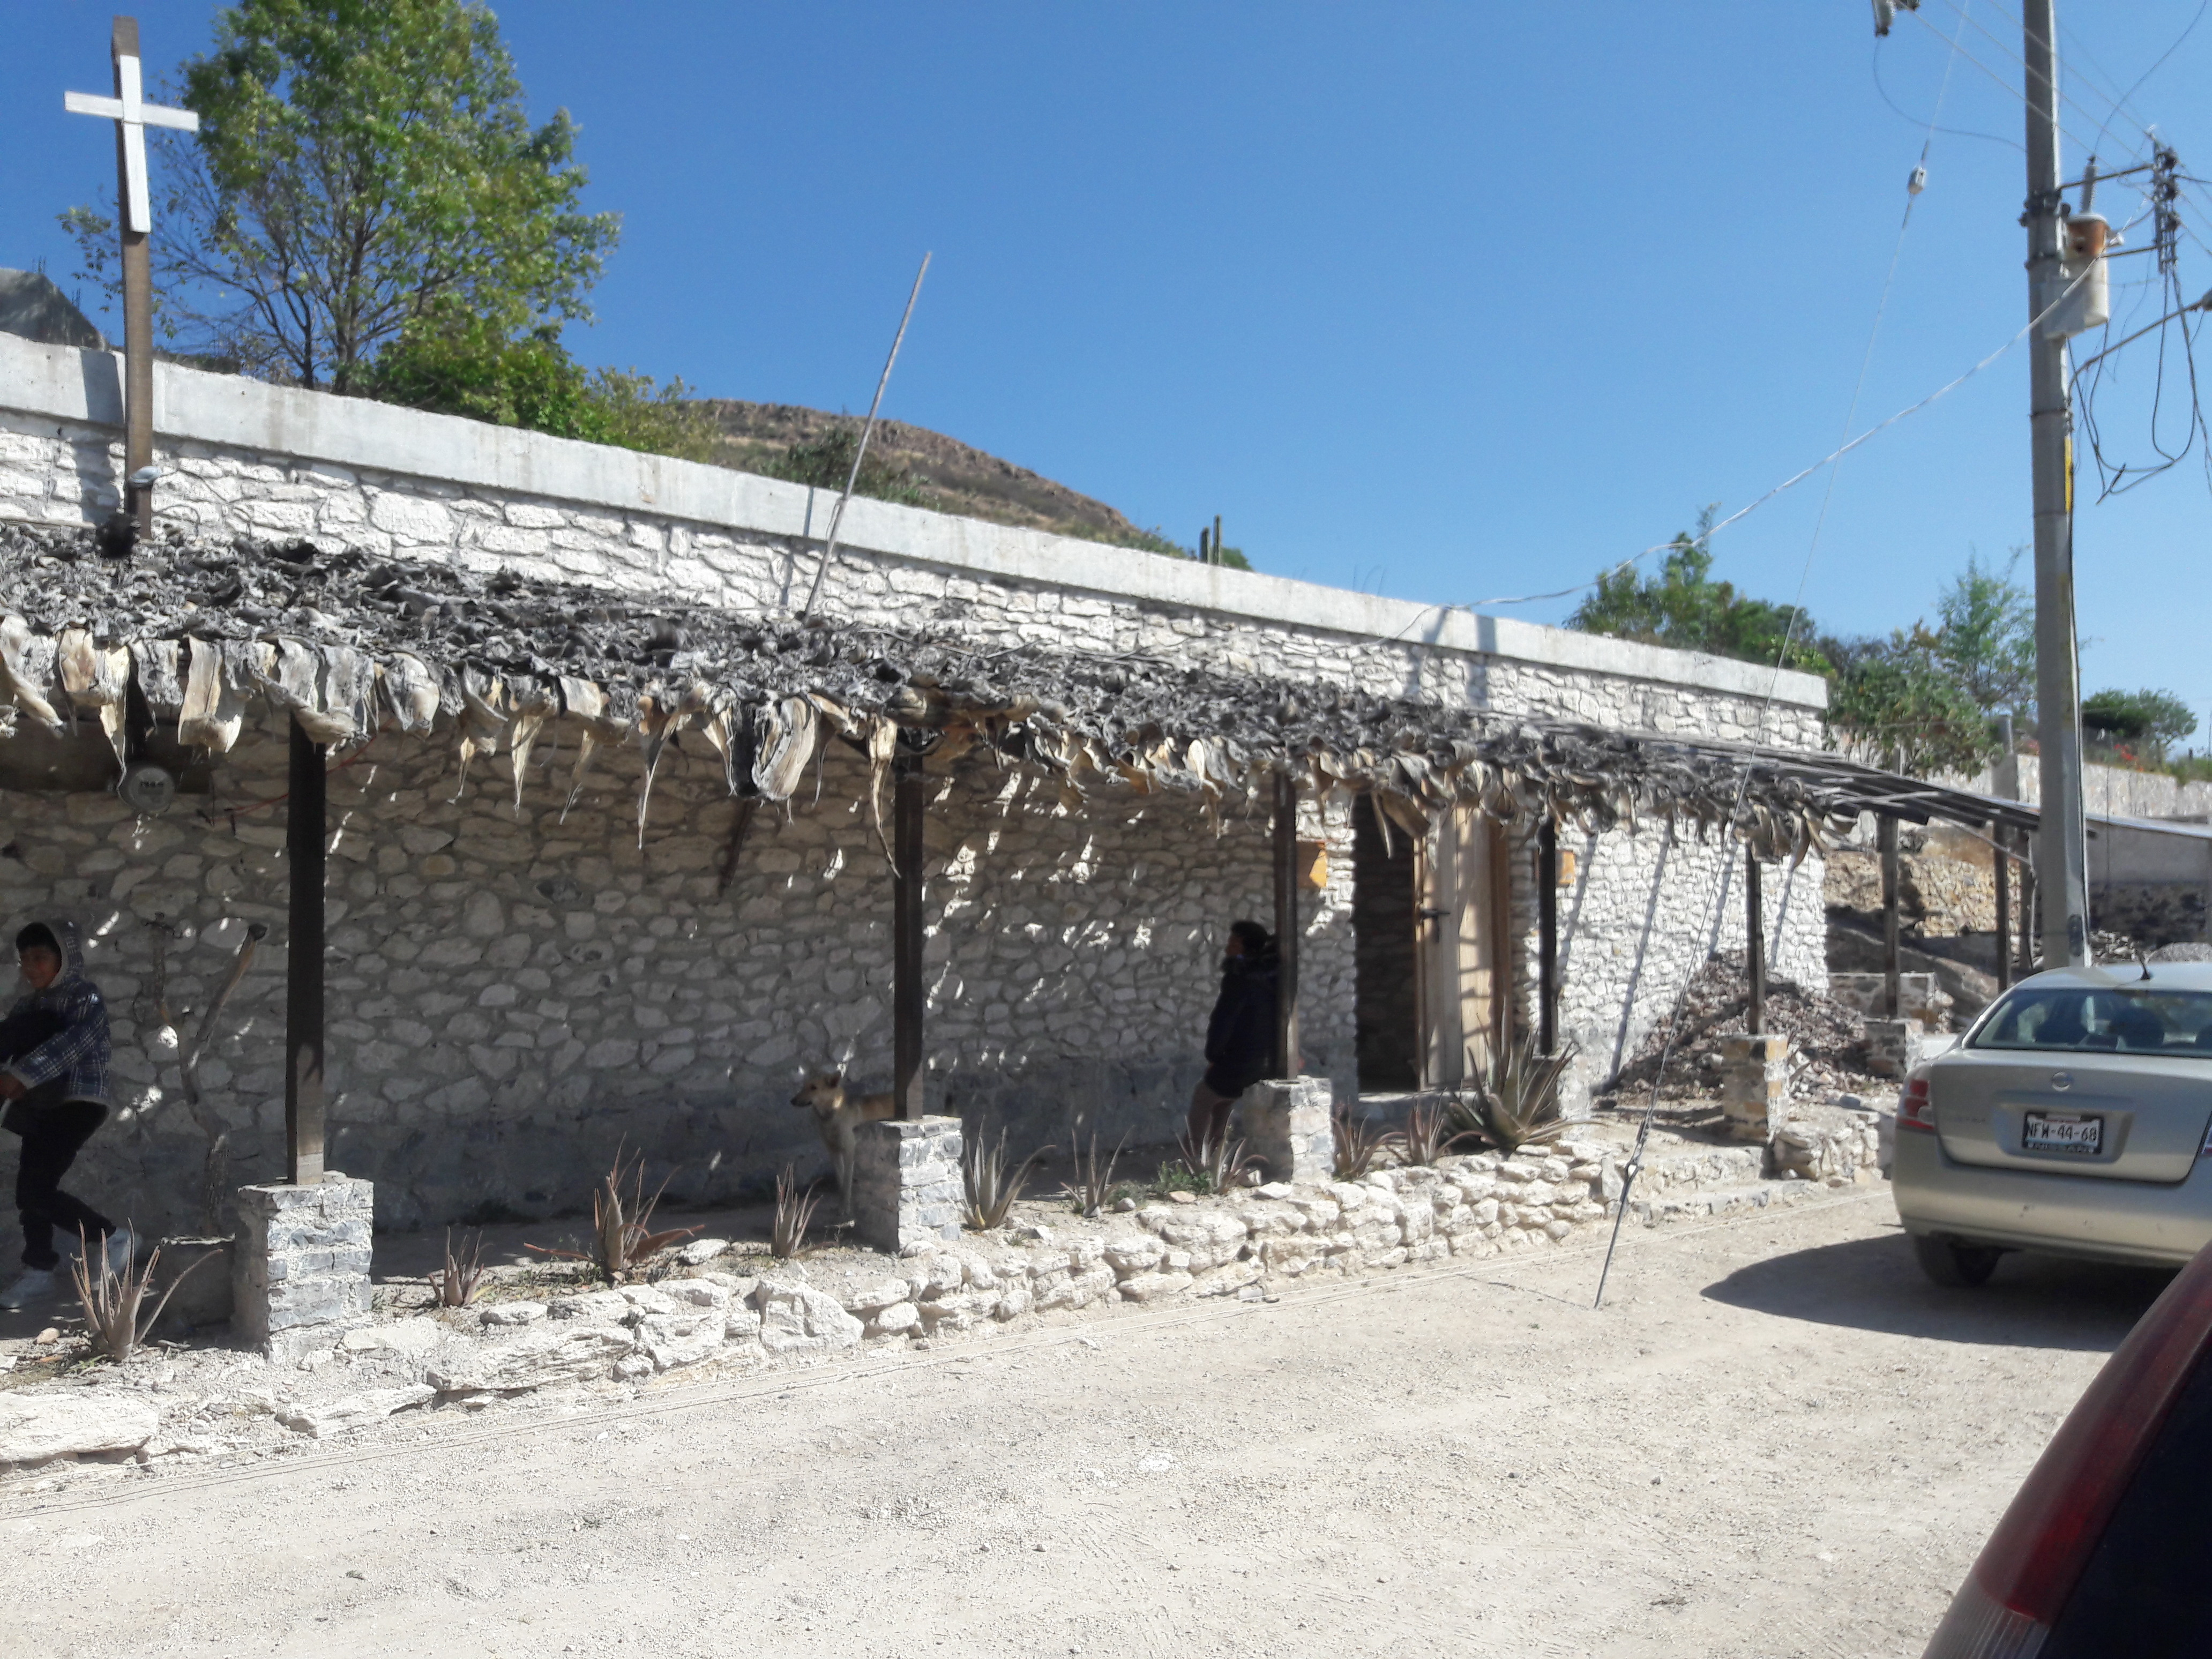
\includegraphics[width=0.8\textwidth]{../../imagenes/Xido_Ngu.jpg}
    \caption{Fachada principal taller \emph{Xido Ngu}}
\end{figure}

Esta manera de pensar se ve reflejada en todos las personas pertenece no solo a Plácido sino a todo su grupo, ya que todos y cada uno reflejan el deseo de cuidar lo tradicional y cuidar su cultura.

Sin embargo, este es un pensamiento tiene una contra parte muy clara y definida en la comunidad donde se habitan, ya que es una comunidad cuyos habitantes desean el mejorar, pensando que lo que se ve en el exterior es lo bueno con relación al vivir.

En casos diferentes, la necesidad supera todo lo que tenga que ver con lo tradicional, la cultura y el origen, ya que estos aspectos solo pueden retomarse una vez que las demás necesidades hayan sido satisfechas. Siendo este el caso de Plácido, el cual, planeaba regresar de Estados Unidos con la intención de construir algo completamente diferente al taller, como la mayoría de los habitantes que regresan del extranjero lo piensan, el construir con materiales industrializados como el block, el tabique y el concreto.

Siendo los sistemas constructivos tradicionales parte de la historia de nuestro país, de las comunidades y su evolución a lo largo de los años así como de testigo de sus costumbres mas arraigadas, con una importancia tanto en su visión del mundo, la vivienda es parte fundamental en las relaciones personales, siendo el núcleo de desenvolvimiento de las personas, un lugar único para cada ser y familia, símbolo de protección y que en ocasiones, tiene un sentir propio, lleno de vida. ``Al entrar en la construcción de adobe, sienten que las acoge, que tiene vida, que tiene mucha historia de los abuelos, de sus generaciones pasadas''\citep{jeronimas}.

\begin{figure}[ht]
    \center
    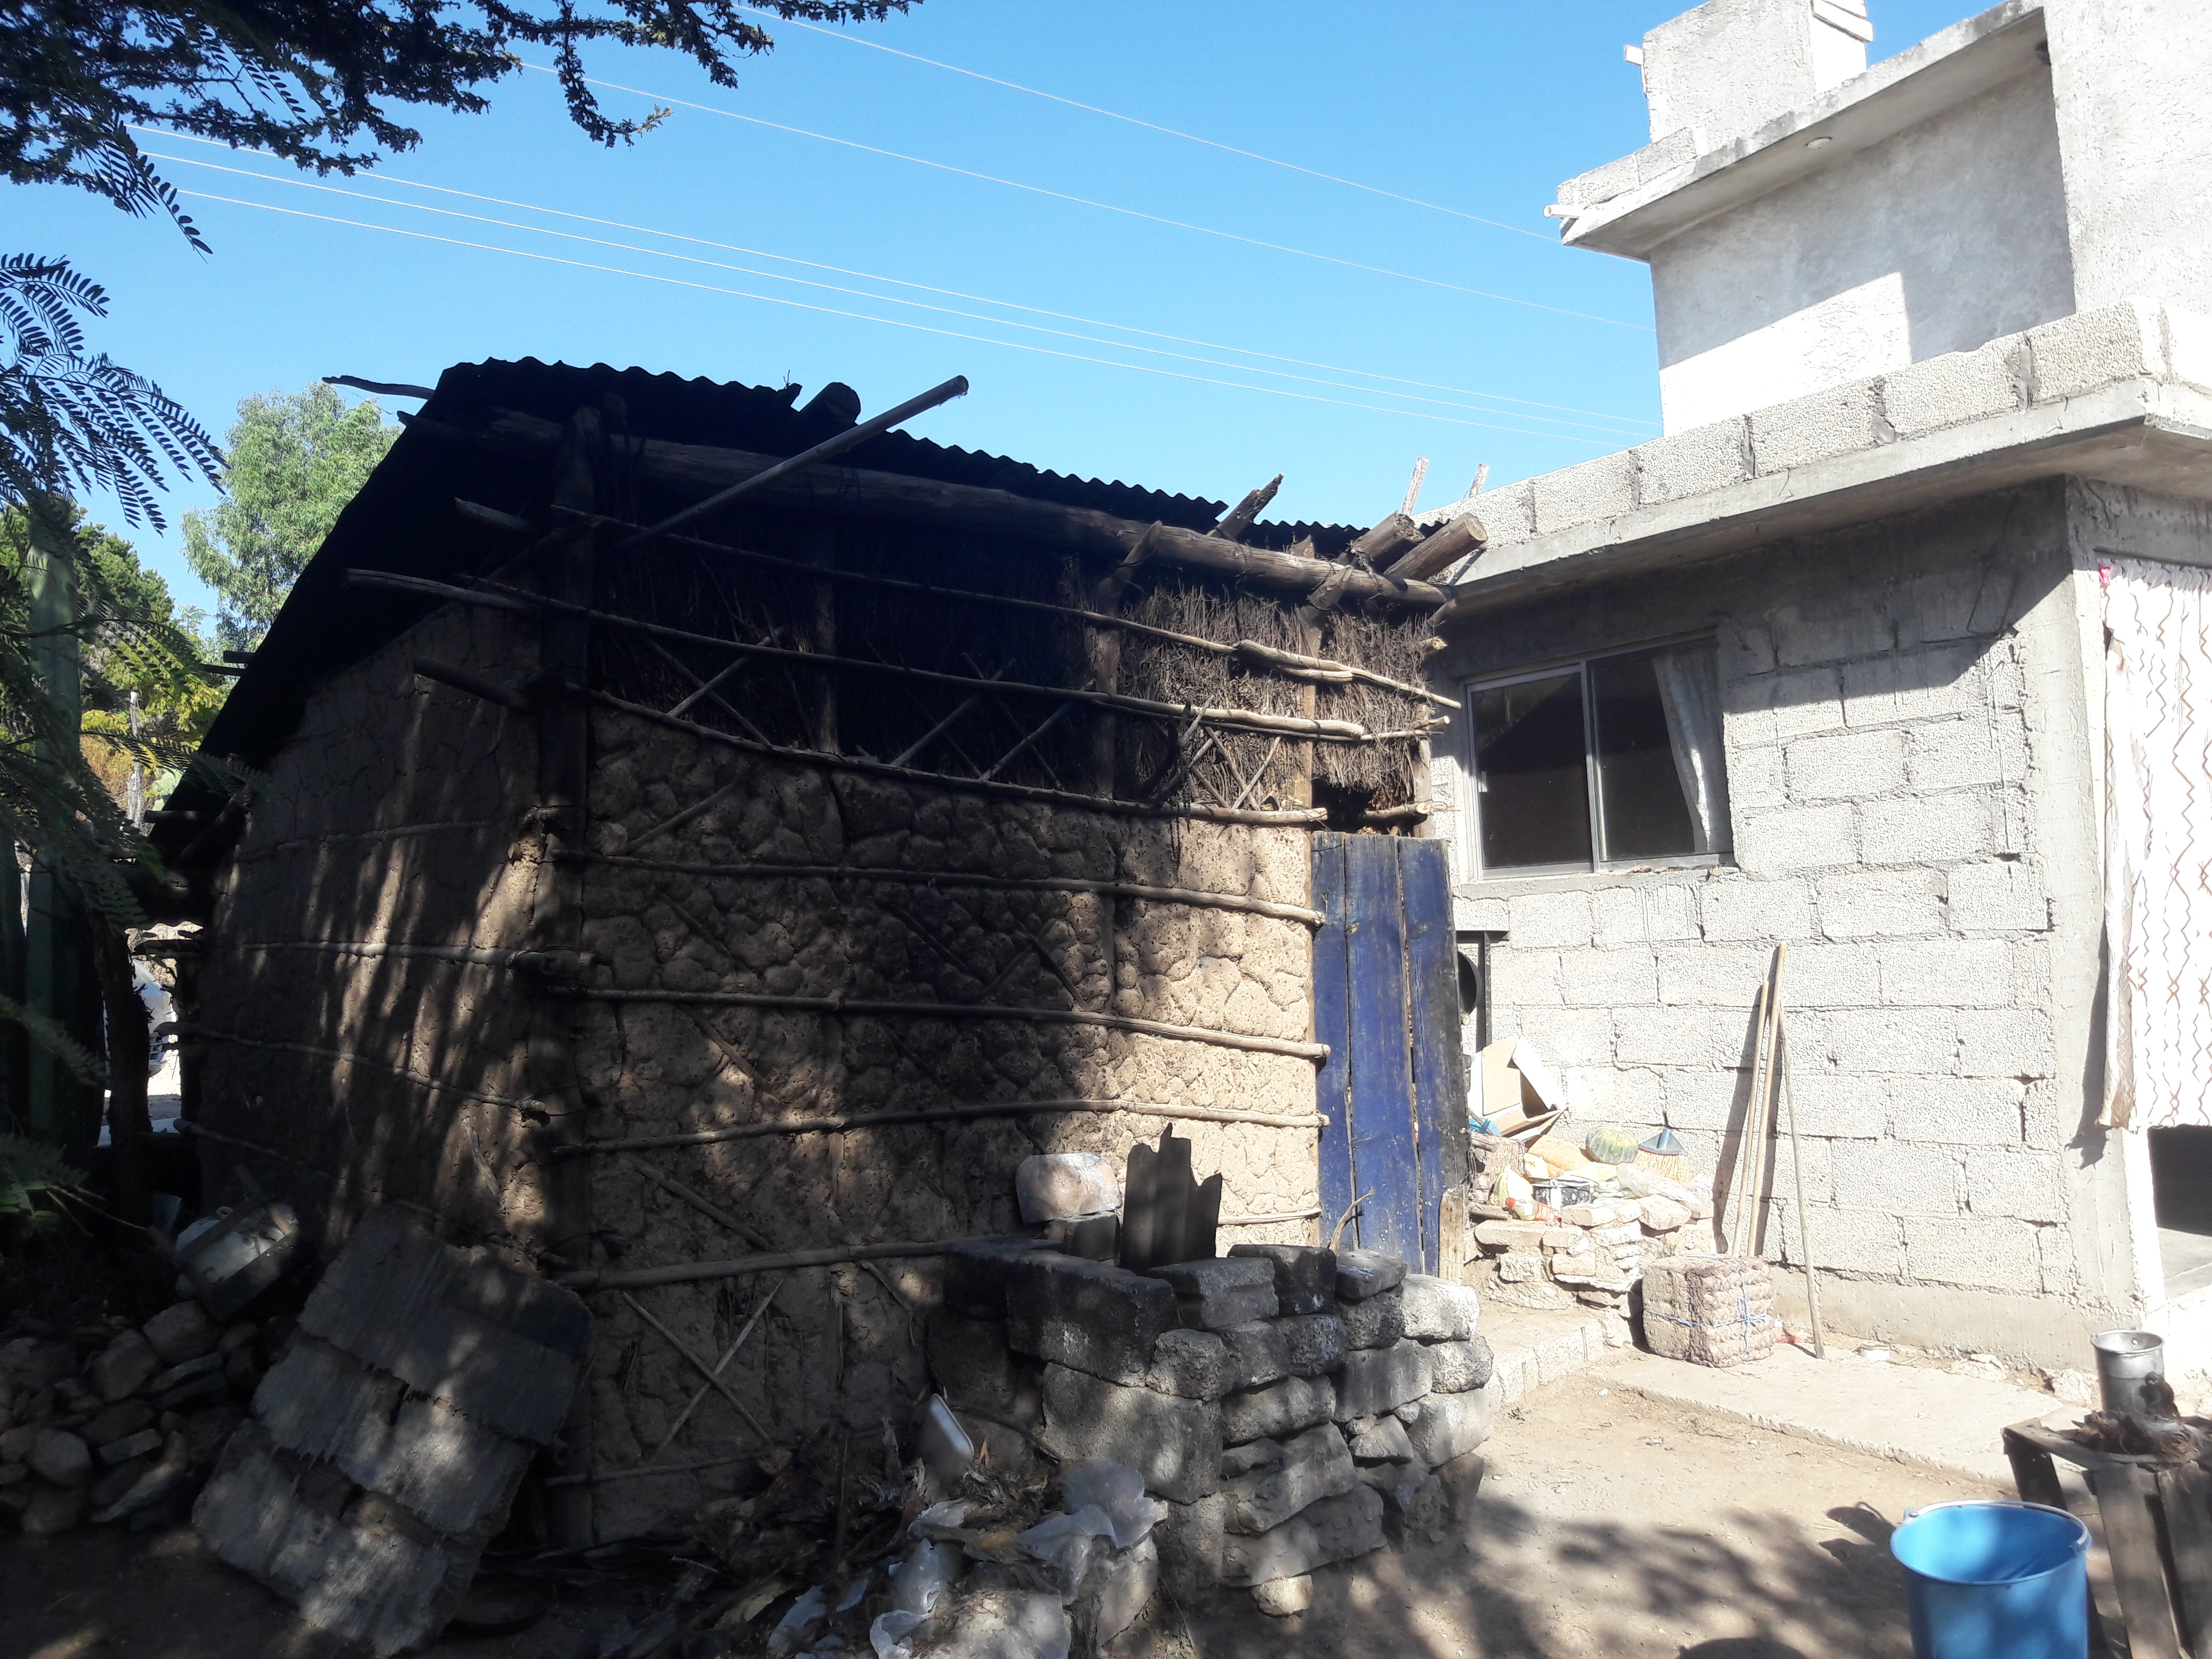
\includegraphics[width=0.8\textwidth]{../../imagenes/Contraste.jpg}
    \caption{Contraste entre vivienda tradicional y vivienda moderna}
\end{figure}

Teniendo en cuenta que la vivienda en todos los lugares del mundo a sido parte de cambios sociales y culturales, en donde las personas al igual que sus hogares, cambian para adaptarse a las nuevas formas de vida, junto con la globalización, hay lugares donde el cambio acelerado de estas formas de vida está causando que las personas no puedan ir a su ritmo y se vean obligadas a elegir entre su forma actual de vida o tener la necesidad de cambiar drásticamente a lo nuevo, lo cual está generando que las costumbres, forma de desenvolverse en el territorio y sus diferentes interacciones en los niveles sociales como vivienda, comunidad y territorio se vean afectadas de igual manera.

Existen instituciones que desde hace tiempo se dedican a buscar y salvaguardar este tipo de sistemas constructivos, y esta investigación busca de igual manera ayudar con la documentación y experiencias a este tipo de instituciones, para que su acercamiento no sea desde cero y que encuentren una directriz que las ayude a delimitar sus lugares de estudio o a conocer lugares específicos donde estas tradiciones sigan vivas y puedan crecer enormemente.

\begin{figure}[ht]
    \center
    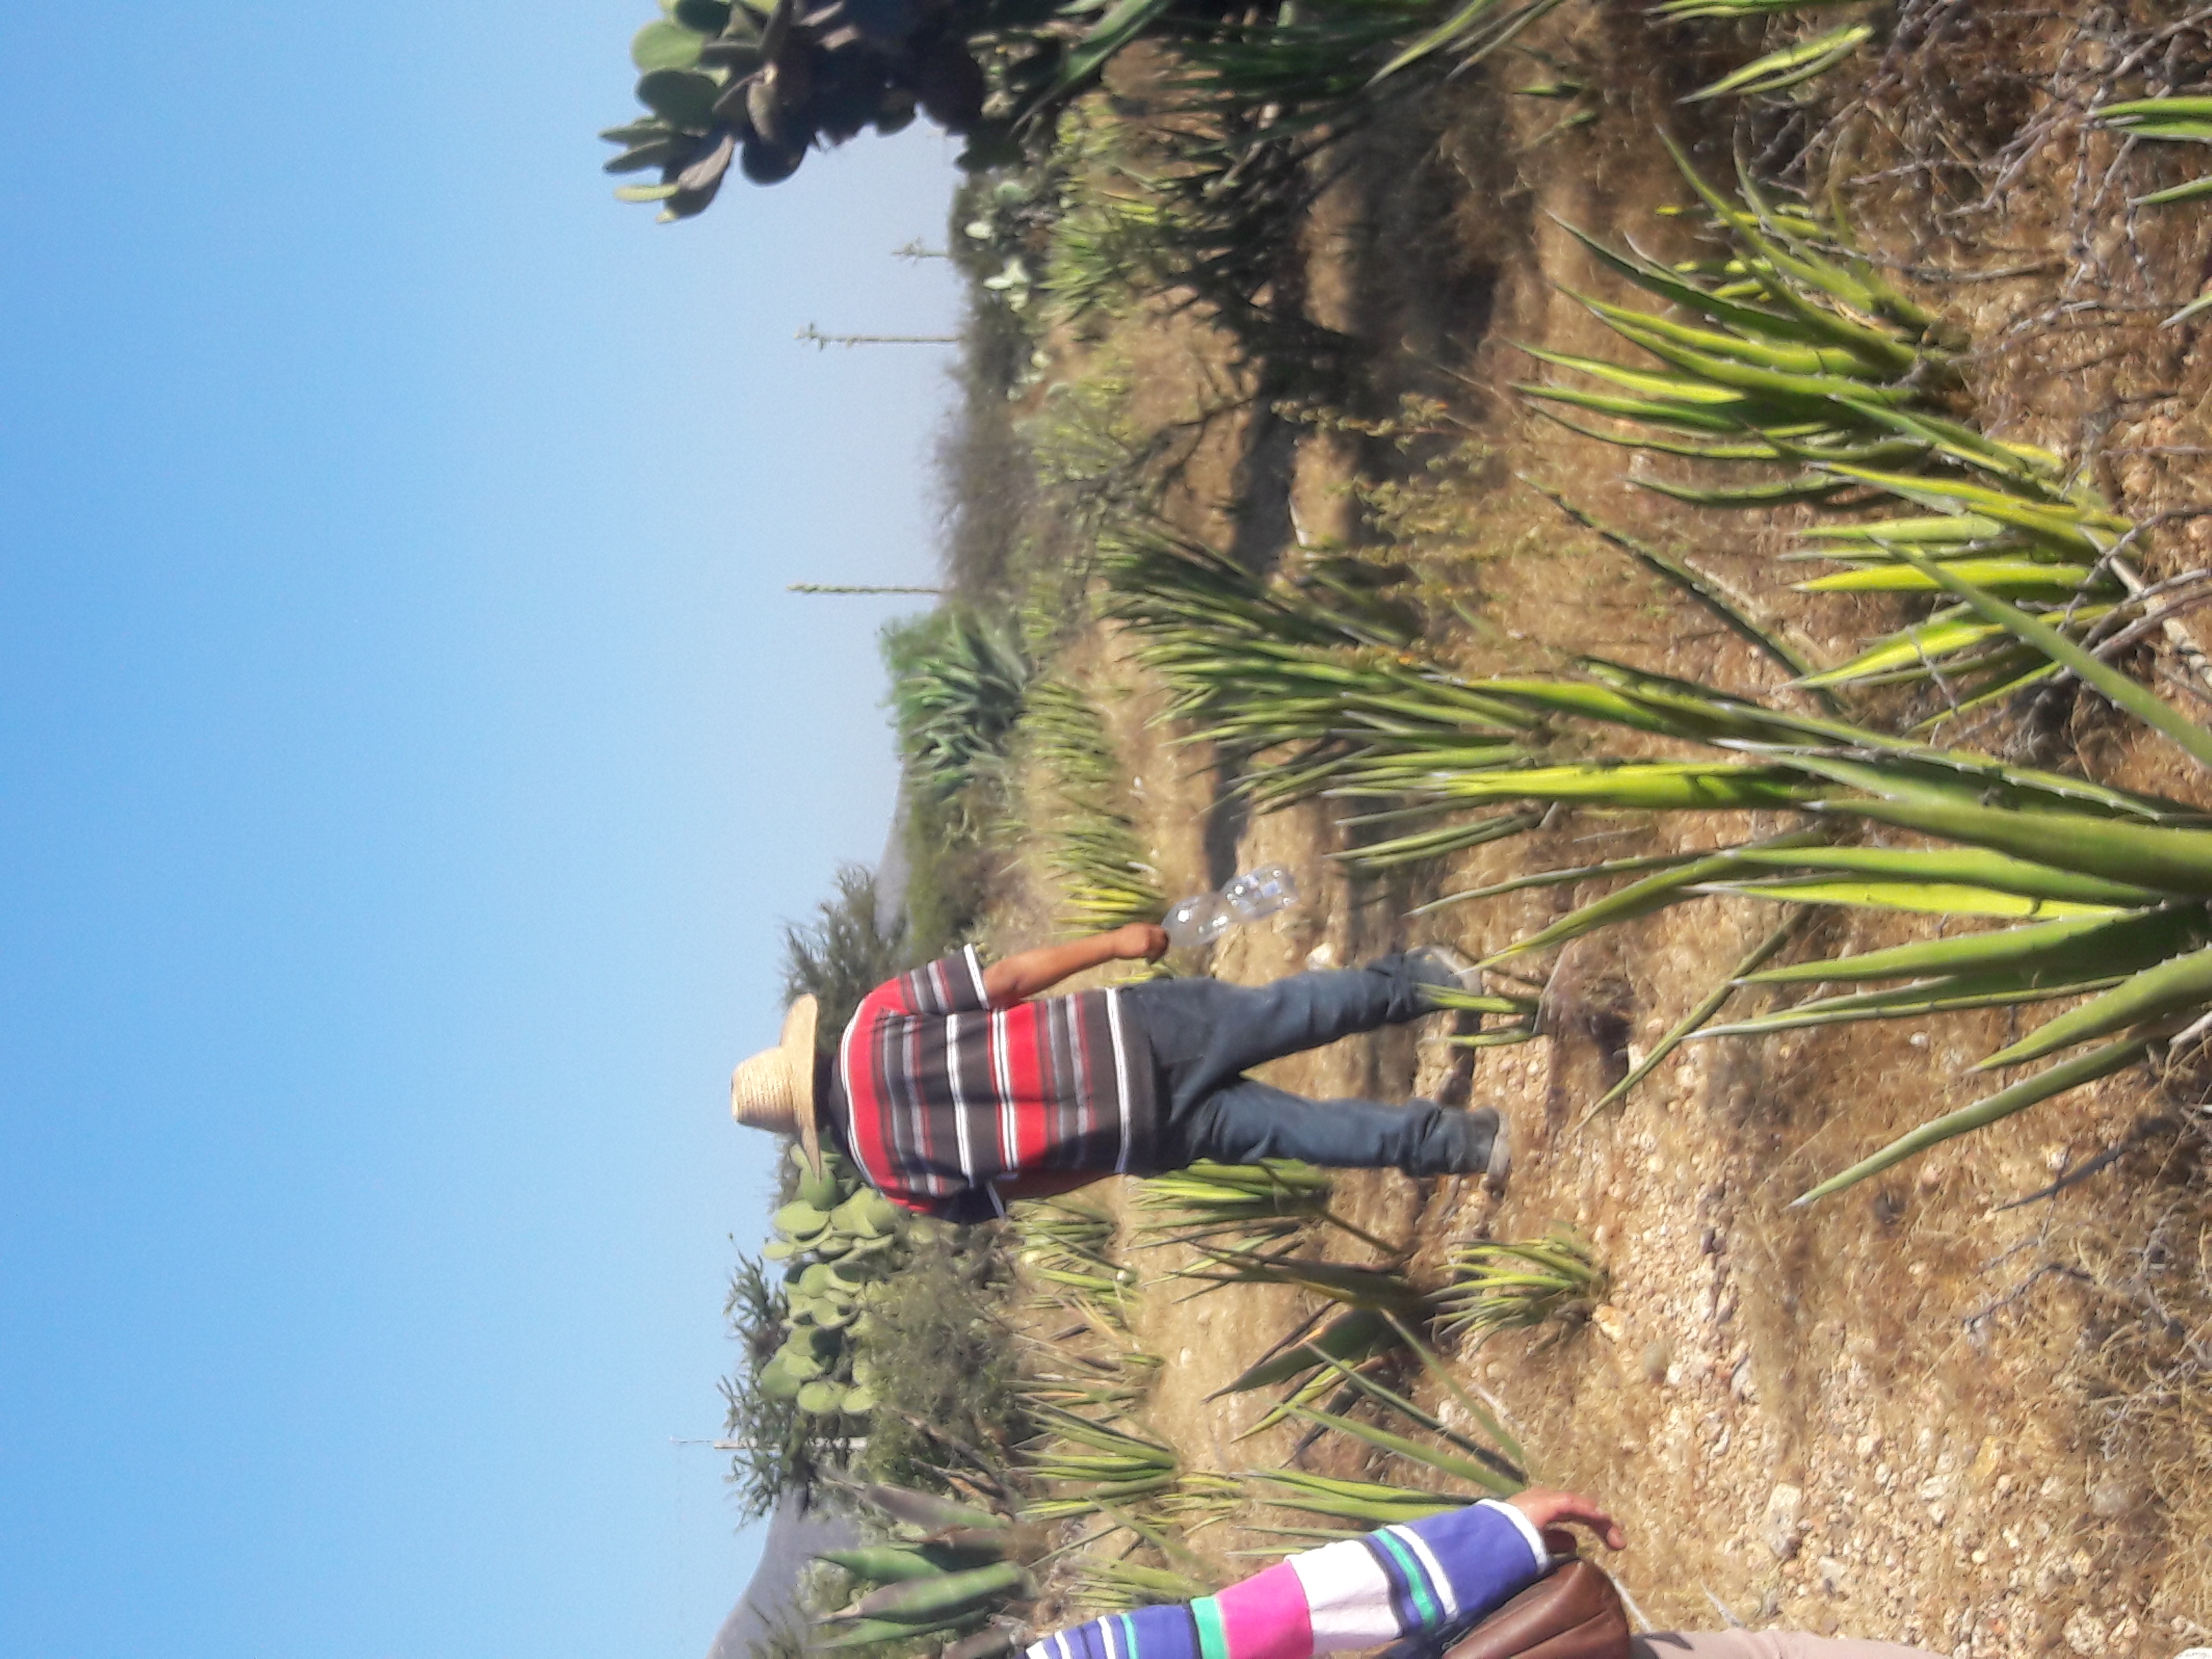
\includegraphics[width=0.8\textwidth, angle=-90]{../../imagenes/placido.jpg}
    \caption{Plácido Paloma en su campo de cucharilla}
\end{figure}
